\chapter{CERN} \label{chap:CERN}
	
	Il \ac{CERN}, anche noto come Organizzazione Europea per la Ricerca sul Nucleare, è l'organizzazione che opera il più grande laboratorio di fisica delle particelle al mondo.
	
	Venne istituito il 29 Settembre 1954 da una serie di stati fondatori nei pressi di Ginevra, a cavallo del confine franco-svizzero. Al momento, il CERN vanta un totale di 21 stati membri, dei quali soltanto Israele non europeo.
	
	\begin{figure}[h!]
		\begin{center}
			
\includegraphics[scale=0.1]{cern_logo.jpg}
		\end{center}
		\caption[Logo del CERN]{Logo del CERN.}
		\label{fig:cern_logo}
	\end{figure}
	
	Col termine \ac{CERN} si indica spesso il laboratorio stesso che, al 2013, contava 2\textquotesingle513 membri staff e circa 12\textquotesingle313 tra fellow, collaboratori associati e studenti, rappresentando un totale di 608 università e 113 nazionalità.
	
	L'obiettivo principale del \ac{CERN} è quello di fornire acceleratori di particelle ed altri strumenti e infrastrutture necessarie per le ricerche di fisica delle alte energie.
	
	Al \ac{CERN} è stata anche proposta e sviluppata una prima implementazione del \aclu{WWW}. All'interno del sito di Meyrin del \ac{CERN} è presente il Data Center principale, che vanta una serie di infrastrutture per l'elaborazione di dati, con lo scopo principale di analizzare dati sperimentali provenienti dal complesso degli acceleratori. Per questo motivo, e per il fatto che questi dati dovevano essere disponibili ed analizzabili da molti altri centri di ricerca, spesso molto distanti, il Data Center di Meyrin divenne un grandissimo centro di smistamento dati, formando una vasta rete tra i vari centri di ricerca.
	
	\section{Breve storia} \label{sec:C;storia}
	
		La convenzione che istituì il \ac{CERN} venne ratificata il 29 Settembre 1954 da 12 stati dell'Europa occidentale.
		
		L'acronimo \ac{CERN}, in origine, indicava la sigla francese \emph{\aclu{CERN}} (Consiglio Europeo per la Ricerca sul Nucleare), che rappresentava il consiglio provvisorio istituito nel 1952 dai 12 stati fondatori per la costruzione di un laboratorio di ricerca di fisica nucleare europeo. Quando il consiglio venne sciolto nel 1954 il nome cambiò all'attuale Organizzazione Europea per la Ricerca sul Nucleare (in francese, \emph{\aclu{OERN}}). In quest'occasione si decise di mantenere la vecchia sigla \ac{CERN} al posto della, più brutta e meno d'impatto, sigla \ac{OERN}. Il fisico Heisenberg stesso si pronunciò sul fatto che l'acronimo sarebbe dovuto rimanere \ac{CERN} anche se il nome non lo era più.
		
		Il \ac{CERN} viene considerato un laboratorio di pace in quanto grazie ad esso persone provenienti da tutto il mondo hanno la possibilità di incontrarsi, discutere e collaborare su diversi progetti. Grazie al \ac{CERN} riescono a lavorare assieme anche persone provenienti da stati in guerra tra loro, come ad esempio Israele e Palestina. Inoltre, il \ac{CERN} venne istituito circa 10 anni dopo la costruzione della bomba atomica come conseguenza principale della II guerra mondiale.
		
		\subsection{Principali scoperte scientifiche} \label{subsec:C;s;principali_scoperte_scientifiche}
		
			In origine, lo scopo principale del \ac{CERN} era quello di studiare i nuclei atomici, ma ben presto l'attenzione si volse verso lo studio della fisica delle alte energie, in particolare all'interazione tra le particelle subatomiche.
			
			\paragraph{1973}Nel 1973 venne scoperta, grazie alla camera a bolle Gargamelle, una particolare interazione tra particelle subatomiche, detta \textit{corrente debole neutra} (Figura \ref{fig:corrente_debole_neutra}) che, nel 1979, permise l'attribuzione del Premio Nobel per la Fisica ad Abdus Salam, Sheldon Glashow e Steven Weinberg, che teorizzarono quest'interazione in passato.
			
			\begin{figure}[h!]
				\begin{center}
					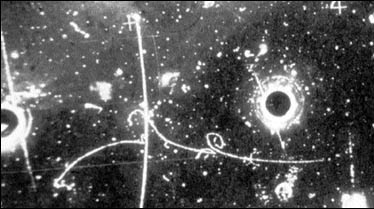
\includegraphics[scale=0.6]{neutral_current.jpg}
				\end{center}
				\caption[Corrente debole neutra]{L'evento di corrente debole neutra osservato con Gargamelle.}
				\label{fig:corrente_debole_neutra}
			\end{figure}
			
			\paragraph{1983}Nel 1983 venne fatta un'altra importantissima scoperta di fisica delle particelle, ovvero la scoperta dei bosoni W e Z. La teorizzazione di questi bosoni fu una conseguenza quasi immediata dell'osservazione della corrente debole neutra, ma prima di poter osservare direttamente queste particelle subatomiche si dovette aspettare di avere un acceleratore di particelle abbastanza potente da produrle. Il primo acceleratore in grado di fare ciò installato al \ac{CERN} fu il \ac{SPS}, che permise, nel Gennaio del 1983 di osservare chiare tracce del bosone W. Gli esperimenti principali furono due, condotti in parallelo, e vennero chiamati UA1 (condotto da Carlo Rubbia) e UA2 (condotto da Pierre Darriulat). I due esperimenti osservarono anche, nel Maggio 1983, i bosoni Z, grazie all'introduzione della tecnica del raffreddamento stocastico introdotta da Simon van der Meer. Nel 1984, la fondazione Nobel, attribuì a Rubbia e Van der Meer il Premio Nobel per la Fisica per l'insostituibile sforzo messo in queste ricerche.
			
			\paragraph{1989}Nel 1989 venne confermato sperimentalmente, utilizzando il \acr{LEP}, che il numero di famiglie di particelle con neutrini leggeri è 3, numero consistente con il Modello Standard.
			
			\begin{figure}[h!]
				\begin{center}
					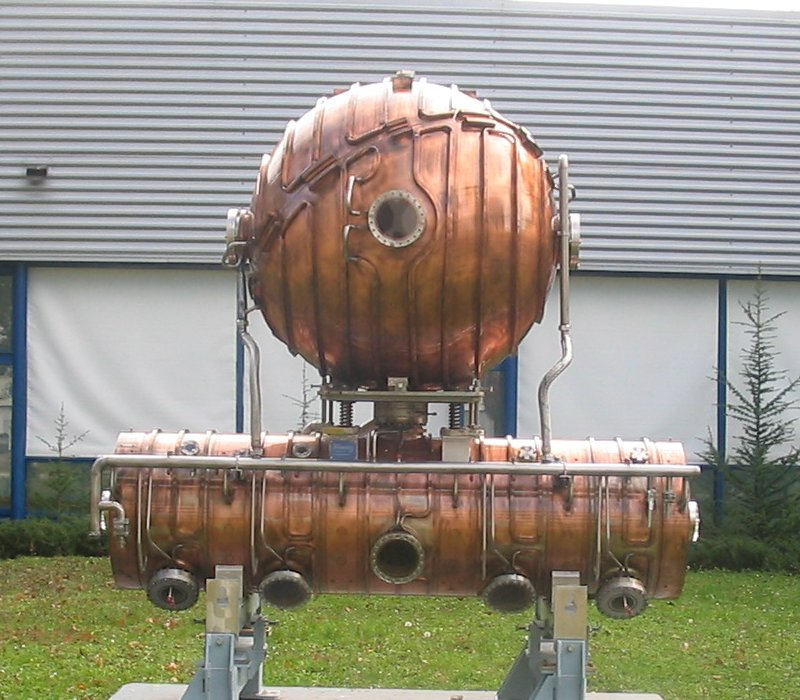
\includegraphics[scale=0.3]{lep_rf.jpg}
				\end{center}
				\caption[Cavità RF del LEP]{Una cavità RF del LEP esposta al Microcosm del CERN.}
				\label{fig:lep_rf}
			\end{figure}
			
			\paragraph{1992}Nel 1992 venne conferito il Premio Nobel per la Fisica a Georges Charpak per ``per l'invenzione e lo sviluppo dei rivelatori di particelle, in particolare della camera proporzionale a multifili''.
			
			\paragraph{1995}Nel 1995 vennero, per la prima volta nella storia, creati atomi di anti-idrogeno grazie all'esperimento PS210 realizzato al \acr{LEAR}. Questi atomi di anti-idrogeno erano molto instabili e si distrussero subito dopo la creazione, ma non senza produrre un segnale elettrico unico, indice che erano effettivamente stati creati atomi di anti-idrogeno.
			
			\paragraph{1999}L'esperimento NA48 dimostrò, nel 1999, la violazione della simmetria \acr{CP}. L'esperimento fu lanciato nel 1990 come successore dell'esperimento NA31 con lo specifico scopo di dimostrare la violazione della simmetria \ac{CP}, la quale afferma che le leggi della fisica dovrebbero rimanere le stesse quando una particella viene sostituita con la sua anti-particella (simmetria di coniugazione di carica, C) e le coordinate spaziali invertite (simmetria di parità, P).
			
			\paragraph{2010}Nel 2010 un gruppo di ricercatori guidati dal fisico Jeffrey Hangst riuscì ad isolare 38 atomi di anti-idrogeno per circa un decimo di secondo, mentre nel 2011 si riuscì a mantenere degli atomi di anti-idrogeno per più di 15 minuti, in modo da poter studiare più a fondo l'antimateria e le sue proprietà.
			
			\paragraph{2012}Infine, nel 2012, venne finalmente osservato un bosone di massa circa $125 \; \sfrac{GeV}{c^2}$ consistente con il tanto cercato bosone di Higgs. Questo bosone venne teorizzato più di 40 anni fa dai ricercatori Peter Higgs e François Englert ed ha una grande importanza per la fisica delle particelle in quanto la sua esistenza può spiegare come mai alcune particelle hanno massa. L'osservazione definitiva del bosone di Higgs avvenne il 4 Luglio 2012, sfruttando le collisioni prodotte dall'\ac{LHC}, e venne osservato in contemporanea dai due esperimenti \ac{CMS} e \ac{ATLAS}. Questa importantissima scoperta portò al conferimento del Premio Nobel per la Fisica, il 10 Dicembre 2013, ai ricercatori Higgs e Englert.
			
		\subsection{Il CERN e l'informatica} \label{subsec:C;s;informatica}
		
			Il primo computer arrivò al \ac{CERN} nel 1959 e da allora i fisici iniziarono ad utilizzare sempre più gli strumenti informatici per le loro analisi. Un elemento importante in questo contesto fu l'italiano Paolo Zanella, capo del dipartimento \acr{IT} per 13 anni, dal 1976 al 1989.
			
			Gli esperimenti condotti al \ac{CERN} producevano una mole di dati sempre più grande, tale da rendere impossibile la sola analisi ``a mano''. Nel tempo, venne sperimentato il collegamento fra più calcolatori portando all'utilizzo delle prime reti di calcolatori. Presto, al \ac{CERN} si formò uno dei più grandi centri di calcolo in Europa. Più recentemente si sono iniziate a sviluppare al \ac{CERN} tecnologie per il grid computing, con progetti come \ac{EGEE} o LHC Computing Grid.
			
			\begin{figure}[h!]
				\begin{center}
					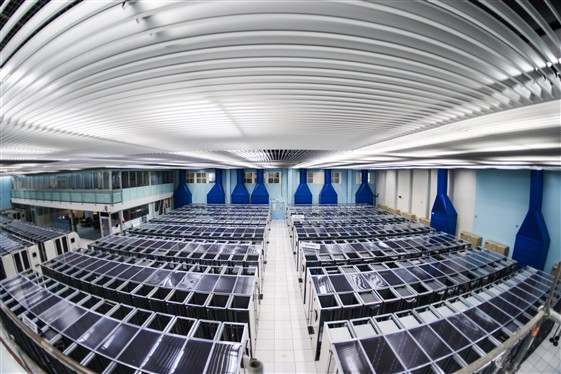
\includegraphics[scale=0.5]{data_center.jpg}
				\end{center}
				\caption[Server Room del Data Center]{L'interno della Server Room del Data Center nel sito di Meyrin.}
				\label{fig:data_center}
			\end{figure}
			
			Il servizio Internet \aclu{WWW} prese vita al \ac{CERN} dal progetto ENQUIRE, condotto da Tim Berners-Lee nel 1989 e Robert Cailliau nel 1990. Nel 1995 Berners-Lee e Cailliau vennero premiati dalla \acr{ACM} per l'indispensabile contributo allo sviluppo del \aclu{WWW}. Il progetto era basato sul concetto di ipertesto, ovvero testo riprodotto su display e collegato ad altri testi tramite iperlink. L'obiettivo originale era quello di facilitare lo scambio di informazioni tra i ricercatori per condurre analisi ed esperimenti.
			
			Il primo sito web fu attivato nel 1991 ed il 30 Aprile 1993 il \ac{CERN} annunciò pubblicamente che il Web sarebbe stato libero per tutti.
			
	\section{Il complesso degli acceleratori} \label{sec:C;acceleratori}
	
		Al \ac{CERN} viene utilizzata una serie di acceleratori disposti in sequenza in modo da aumentare l'energia delle particelle prima di essere ridirette agli eventuali esperimenti o all'acceleratore successivo. Il logo stesso del \ac{CERN} (Figura \ref{fig:cern_logo}) è ispirato al complesso degli acceleratori presente.
			
		\begin{figure}[h!]
			\begin{center}
				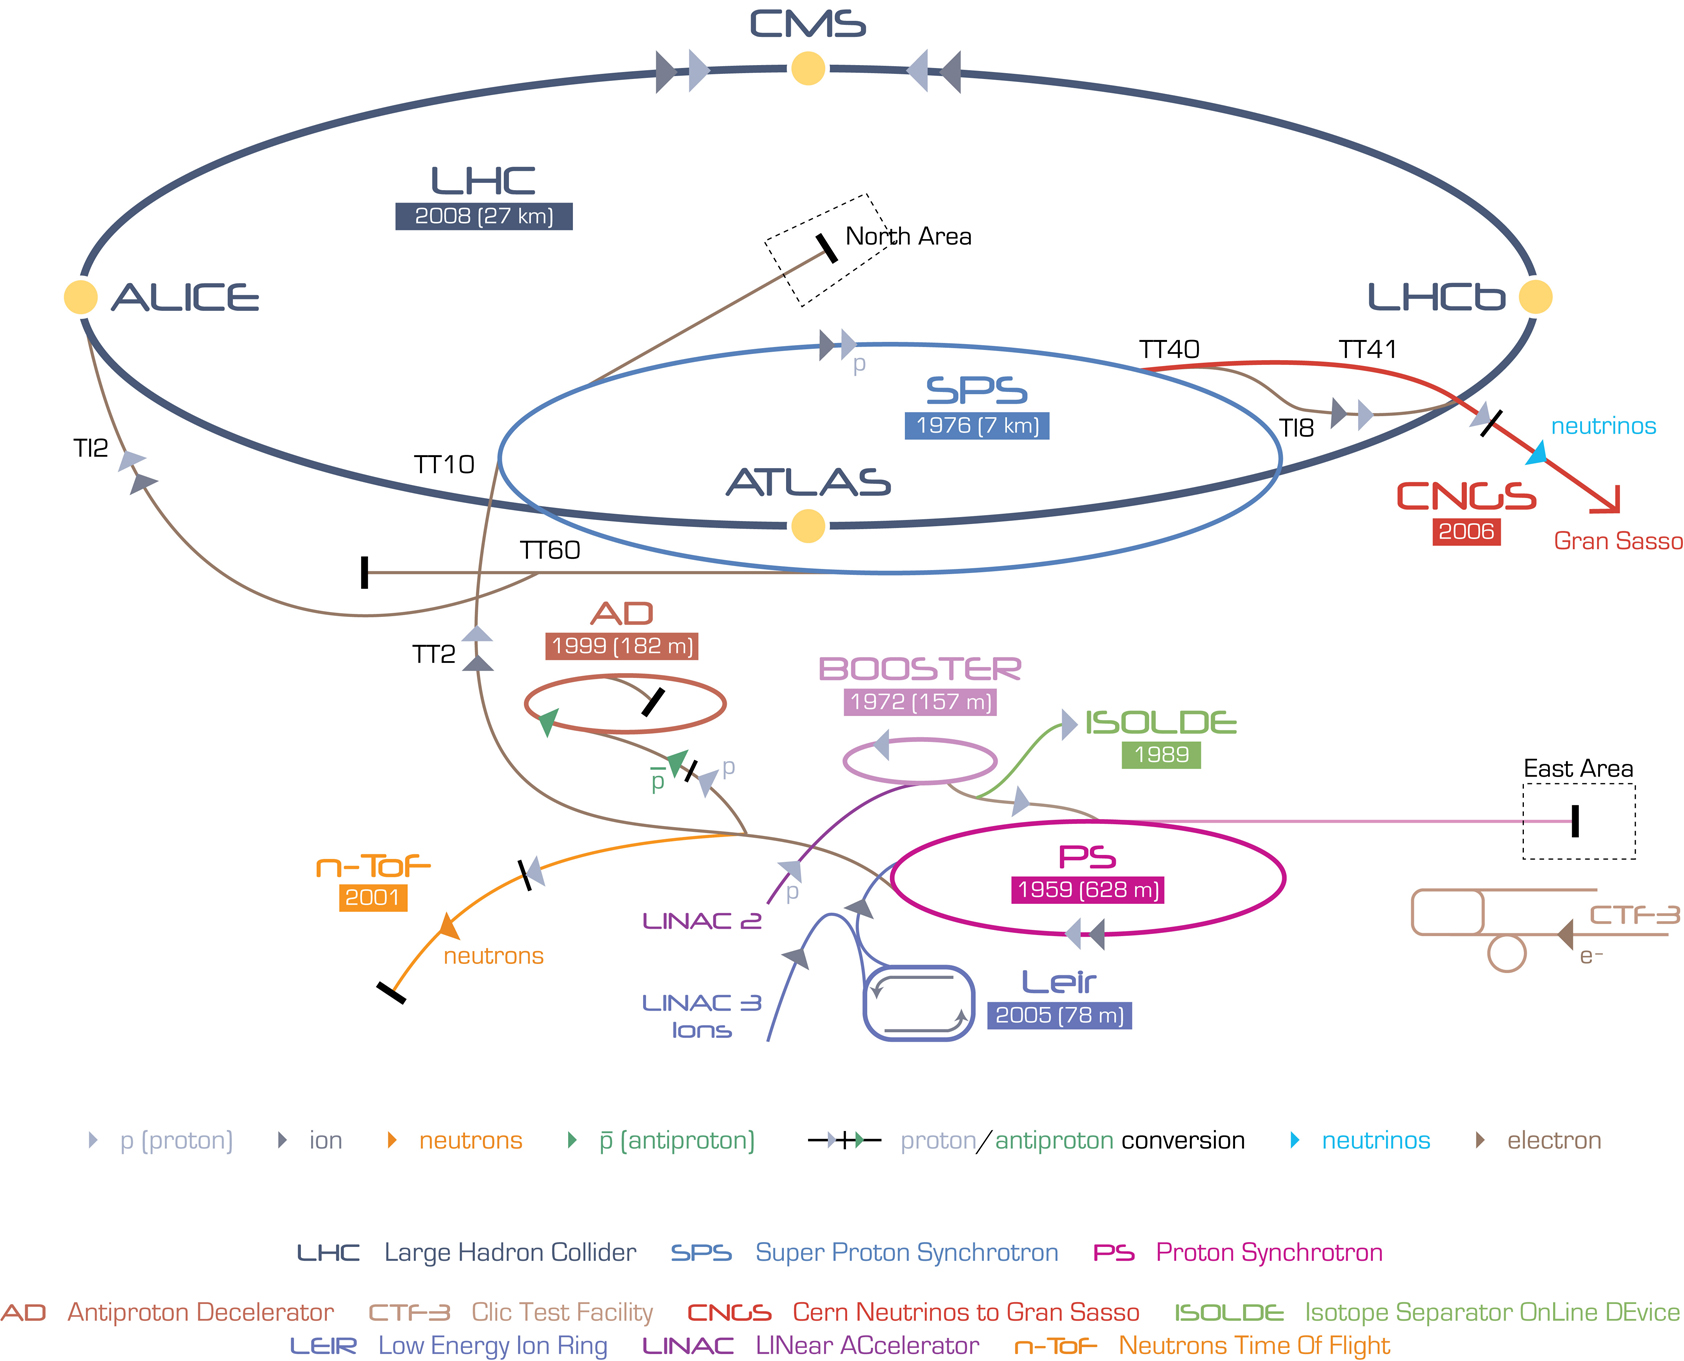
\includegraphics[scale=0.4]{accelerator_complex.jpg}
			\end{center}
			\caption[Complesso degli acceleratori]{Uno schema del complesso degli acceleratori presenti al CERN con legenda.}
			\label{fig:accelerator_complex}
		\end{figure}
		
		I macchinari attualmente attivi al \ac{CERN} sono i seguenti:
		
		\paragraph{Linac2 e Linac3}Questi due acceleratori lineari (\acs{Linac} sta per \aclu{Linac}) generano particelle a bassa energia. Linac2 accelera protoni fino a $50 \; MeV$ per poi iniettarli nel \ac{PSB}, mentre Linac3 genera ioni pesanti a $4.2 \; \sfrac{MeV}{u}$ per iniettarli nel \ac{LEIR}.
		
		\paragraph{Proton Synchrotron Booster}Aumenta l'energia dei protoni prodotti dal Linac2 prima di trasferirli ad altri acceleratori.
		
		\paragraph{Low Energy Ion Ring}Accelera gli ioni pesanti prodotti dal Linac3 prima di trasferirli al \ac{PS}. Questo acceleratore fu commissionato nel 2005 come riconfigurazione del precedente acceleratore, il \ac{LEAR}.
		
		\paragraph{Proton Synchrotron}Accelera le particelle fino a $28 \; GeV$. Fu costruito tra il 1954 ed il 1959 ed è ancora attivo come alimentatore del più potente \ac{SPS}.
		
		\paragraph{Super Proton Synchrotron}Acceleratore circolare installato in un tunnel di 2 Km di diametro ed attivo dal 1976. Fu costruito inizialmente per portare le particelle fino a $300 \; GeV$, per poi essere gradualmente aggiornato fino ai $450 \; GeV$. Questo acceleratore ha i propri esperimenti, al momento \acr{COMPASS} ed NA62, ma veniva anche utilizzato come collisore protoni-antiprotoni e per accelerare elettroni e positroni prima di iniettarli nel \ac{LEP}. Dal 2008 viene invece utilizzato per iniettare protoni e ioni pesanti nell'\ac{LHC}.
		
		\paragraph{On-Line Isotope Mass Separator}Anche indicato con la sigla \acs{ISOLDE}\acused{ISOLDE}, questa struttura viene utilizzata per studiare i nuclei instabili. Ioni radioattivi provenienti dal \ac{PSB} vengono fatti scontrare con un energia tra $1.0$ e $1.4 \; GeV$.
		
		\paragraph{Antiproton Decelerator}Anche noto come \acs{AD}\acused{AD}, serve a ridurre la velocità degli antiprotoni di circa un $10\%$ della velocità della luce per poter studiare l'antimateria.
		
		\paragraph{Compact Linear Collider}Studia la fattibilità di possibili acceleratori lineari futuri.
		
		\subsection{Large Hadron Collider} \label{subsec:C;a;LHC}
			
			L'\ac{LHC} è attualmente il più grande acceleratore di particelle installato al \ac{CERN}, ovvero l'acceleratore principale su cui vengono eseguiti la maggior parte degli esperimenti.
			
			Il tunnel dell'\ac{LHC} è situato 100 metri sotto terra, nella zona tra l'Aeroporto Internazionale di Ginevra e i monti del Giura. Il tunnel ha una circonferenza di circa 27 Km ed era precedentemente occupato dal vecchio acceleratore \ac{LEP}, che venne disattivato definitivamente nel 2000. Gli acceleratori \ac{PS} ed \ac{SPS} vengono utilizzati per pre-accelerare i protoni iniettati nell'\ac{LHC}.
			
			Lungo l'acceleratore sono presenti i suoi sette esperimenti attualmente attivi: \ac{CMS}, \ac{ATLAS}, \acr{LHCb}, \acr{MoEDAL}, \acr{TOTEM}, \acr{LHCf} ed \acr{ALICE}.
			
			\begin{figure}[h!]
				\begin{center}
					\subfloat[][ATLAS]{
						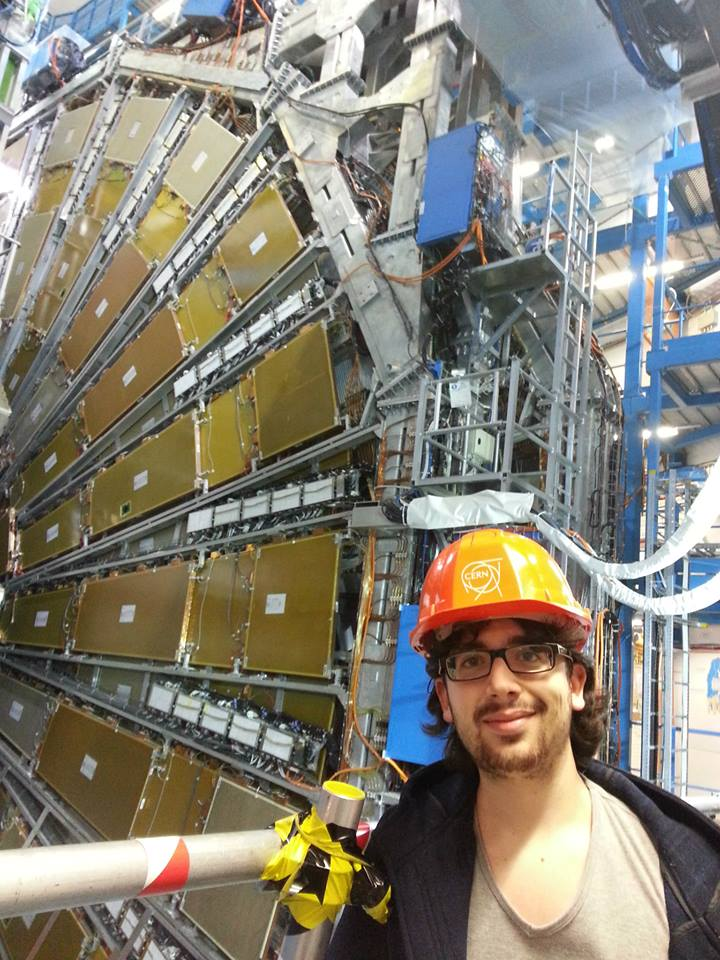
\includegraphics[scale=0.2]{tommaso_atlas.jpg}
					}~
					\subfloat[][CMS]{
						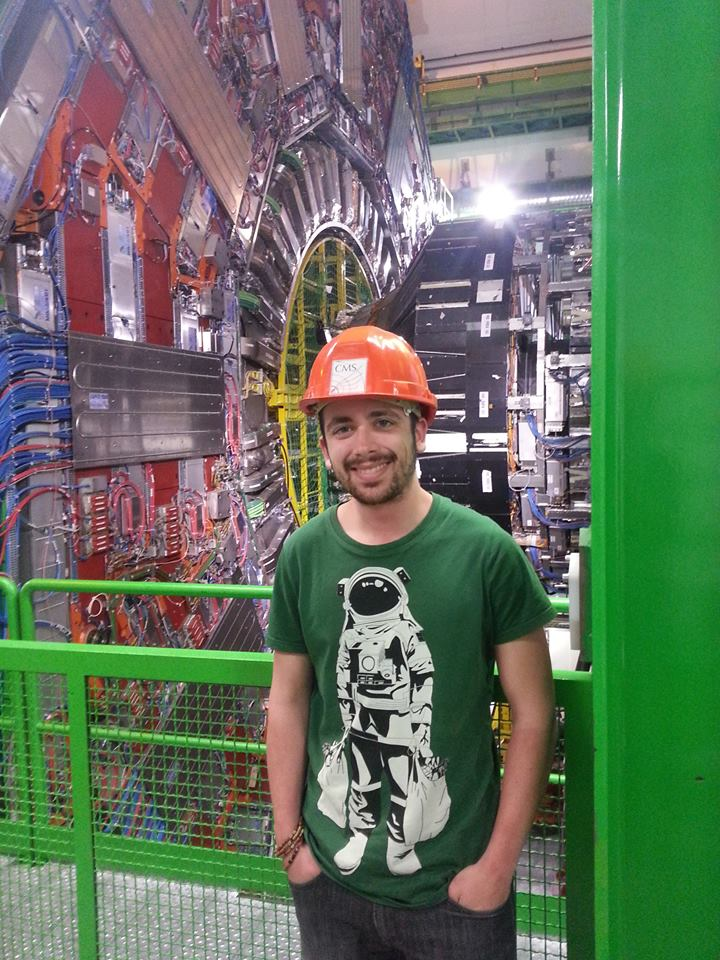
\includegraphics[scale=0.2]{tommaso_cms.jpg}
					}
				\end{center}
				\caption[Visita all'LHC]{Visite ai laboratori sotterranei di alcuni esperimenti dell'LHC.}
				\label{fig:visita_lhc}
			\end{figure}
			
			L'\ac{LHC} iniziò fin da subito a generare una mole enorme di dati da inviare a diversi laboratori sparsi per il mondo in modo da poter eseguire calcoli distribuiti utilizzando una struttura grid dedicata: la LHC Computing Grid.
			
			Il primo fascio di particelle fu iniettato nell'\ac{LHC} nell'Agosto del 2008 ma, a causa di problemi tecnici, non venne riattivato fino al Novembre del 2009. Il 30 Marzo 2010, invece, si verificò la prima collisione tra due fasci di protoni, ognuno alla velocità di $3.5 \; TeV$, generando una collisione di $7 \; TeV$. Dal Marzo 2012 si passò invece a collisioni di $8 \; TeV$ (ovvero $4 \; TeV$ in ogni direzione). Agli inizi del 2013 l'\ac{LHC} venne disattivato per avviare un periodo di manutenzione e aggiornamento della durata di 2 anni. Dai primi mesi del 2015, l'\ac{LHC} è stato finalmente rimesso in funzione per sperimentare le prime collisioni a $13 \; TeV$. Nel Luglio 2012 venne annunciata l'osservazione sperimentale di una particella subatomica consistente con il tanto agognato bosone di Higgs. Nel Marzo 2013 venne confermato dal \ac{CERN} che, a seguito di una serie di analisi condotte sui dati sperimentali, la particella trovata era effettivamente il bosone di Higgs.
	
	\section{Lavoro al CERN} \label{sec:C;lavoro}
	
		Il \ac{CERN} è il risultato di una collaborazione tra stati, università, scienziati e studenti che sono motivati non da un margine di profitto, ma bensì da un impegno a creare e condividere la conoscenza.
		
		Le persone del \ac{CERN}, sia che siano impiegati fissi, che soltanto di passaggio, prendono parte a ricerche e collaborazioni interessanti con persone di tutto il mondo, cercando di risolvere i misteri della fisica o di creare qualcosa di nuovo.
		
		\subsection{Cultura e valori} \label{subsec:C;l;cultura_e_valori}
		
			Al \ac{CERN} vige il Code of Conduct (Codice della Condotta), ovvero una guida su come trattare gli altri colleghi in accordo con i valori del \ac{CERN}. \cite{cern:culture_values}
			
			I cinque valori di base su cui si basa il \ac{CERN} sono:
			
			\paragraph{Integrit\`{a}}Ovvero comportarsi in modo etico, onesto e ritenersi responsabile delle proprie azioni.
			
			\paragraph{Impegno}Dimostrare, durante il proprio lavoro, un alto livello di motivazione e dedizione verso l'organizzazione ed il proprio progetto.
			
			\paragraph{Professionalit\`{a}}Produrre risultati di alta qualità rispettando i limiti di tempo e le risorse previsti per il completamento del lavoro.
			
			\paragraph{Creativit\`{a}}Promuovere l'innovazione nel proprio settore di lavoro e permettere lo sviluppo e l'evoluzione dell'organizzazione.
			
			\paragraph{Diversit\`{a}}Ovvero saper apprezzare le differenze e promuovere l'uguaglianza e la collaborazione.
		
		\subsection{Carriera al CERN} \label{subsec:C;l;carriera}
		
			Il \ac{CERN} ammette un ampio ventaglio di possibilità per fare carriera ed acquisire esperienza lavorativa al suo interno. Ci sono svariati tipi di contratti per tutti i tipi di aspiranti dipendenti o collaboratori \ac{CERN}: contatti di pochi mesi o contratti di anni, contratti per studenti, per laureati o per professionisti, ecc\dots \cite{cern:carreer}
			
			Uno dei principi di assunzione e lavoro al \ac{CERN} è la non rinnovabilità del contratto: ogni tipo di contratto può essere assegnato ad ogni individuo al più una sola volta. Questo serve a garantire la diversità ed il continuo ricambio di personale ed allo stesso tempo formare abitanti degli stati membri con un'esperienza di alto livello.
			
			\paragraph{Studente}In qualità di studente universitario si hanno molte possibilità di lavoro al \ac{CERN} con contratti di Summer, Admin, Technical e Doctoral Student. Il programma di Technical Student (ovvero il programma grazie al quale si è seguito il progetto oggetto di questa tesi) prevede una durata dai 6 ai 12 mesi, con la possibilità di estendere il contratto di 2 ulteriori mesi (risorse permettendo). Questi tipi di contratto permettono agli studenti di fare esperienza sul campo ed affrontare sfide intellettuali con alte possibilità di formazione.
			
			\paragraph{Laureato}I contratti per laureati durano normalmente dai 2 ai 3 anni e permettono una formazione ad alto livello. I principali contratti di questo tipo sono la Fellowship, il Graduate Engineer Training ed il contratto Marie-Curie.
			
			\paragraph{Staff}I contratti di Staff durano 5 anni e sono uno dei più ambiti e prestigiosi tipi di contratto al \ac{CERN} come dipendente effettivo e professionista.
			
			\paragraph{E dopo...}Purtroppo anche i contratti di Staff sono non rinnovabili ed a tempo determinato (5 anni). Tuttavia, verso gli ultimi anni di contratto, il \ac{CERN} dà la possibilità al membro dello Staff di fare domanda per il cosiddetto \ac{IC}, ovvero un contratto di Staff a tempo indeterminato.
	
		\subsection{La struttura generale} \label{subsec:C;l;struttura}
		
			Il consiglio del \ac{CERN} è la più alta autorità dell'intera organizzazione ed è responsabile di tutte le decisioni più importanti. Si occupa di controllare tutte le attività scientifiche, tecniche ed amministrative del \ac{CERN} e di approvare programmi, attività, budget e spese. Il consiglio è composto da 21 stati membri, ognuno dei quali fornisce due delegati come rappresentanti nel consiglio. Uno dei due delegati rappresenterà gli interessi amministrativi del proprio governo, mentre l'altro rappresenterà gli interessi scientifici nazionali. Nel consiglio, ogni stato membro ha a disposizione un solo voto e per la maggior parte delle decisioni si vota per maggioranza. Il consiglio è assistito, nelle sue decisioni, dalla Scientific Policy Commmittee e dalla Finance Committee.
			
			La Scientific Policy Committee (Commissione della Politica Scientifica) valuta i pro e i contro delle attività proposte dai fisici e suggerisce strategie per il programma scientifico al \ac{CERN}. I membri vengono eletti dalla commissione stessa e suggeriti dal consiglio in base ai meriti scientifici, senza distinzioni di nazionalità. La Finance Committee (Commissione della Finanza) è invece composta da rappresentanti delle amministrazioni nazionali e si occupa di gestire i contributi degli stati membri e budget e spese dell'organizzazione.
			
			Il \ac{DG}, eletto dal consiglio ogni 5 anni, si occupa di gestire il laboratorio \ac{CERN}, rispondendo direttamente al consiglio. Il \ac{DG} è assistito da un direttorato e gestisce il laboratorio attraverso una struttura di dipartimenti. Durante i 14 mesi di Techical Student passati al \ac{CERN} il \ac{DG} era il fisico tedesco Rolf-Dieter Heuer, in carica dal 2009. Dal Gennaio 2016, invece, è in carica Fabiola Giannotti, fisica italiana e prima \ac{DG} donna della storia.
			
			Sotto al \ac{DG} si sviluppa la struttura del laboratorio \ac{CERN}, ovvero una struttura piramidale organizzata in dipartimenti. Più in particolare, il \ac{CERN} è suddiviso in otto dipartimenti: \acr{BE}, \acr{EN}, \acr{FP}, \acr{GS}, \acr{HR}, \ac{IT}, \acr{PH}, \acr{TE}. Ogni dipartimento (gestito da un Department Head) è suddiviso in gruppi, che si occupano di settori specifici all'interno dello stesso dipartimento. A loro volta, ogni gruppo (gestito da un Group Leader) si suddivide in sezioni, ognuna delle quali si specializza ulteriormente a seconda del lavoro svolto. Infine, ogni sezione (gestita da un Section Leader) è composta da una serie di progetti. Ad ogni progetto è associato un team il quale, sotto la supervisione di un Project Manager, si occupa di portare a termine il proprio progetto nel modo migliore possibile. \cite{cern:structure}

			\begin{figure}[h!]
				\begin{center}
					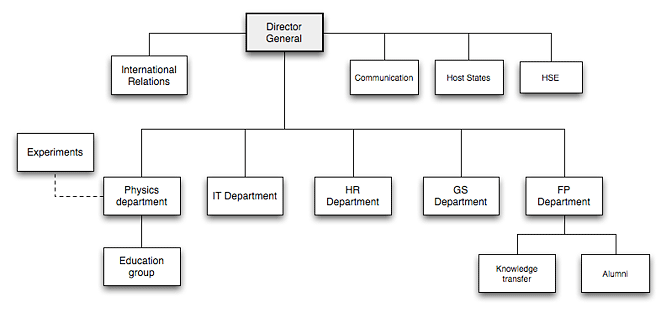
\includegraphics[scale=0.5]{cern_organogram}
				\end{center}
				\caption[Organigramma del CERN]{Organigramma ad alta granularità dell'organizzazione CERN.}
				\label{fig:cern_organogram}
			\end{figure}
			
			\paragraph{Indico}Il progetto Indico, oggetto di questa tesi, è così collocato all'interno della struttura del \ac{CERN}: \ac{IT} - \acs{CIS} - \acs{AVC} - Indico. Indico fa quindi, innanzitutto, parte del dipartimento \ac{IT}, ovvero il dipartimento dei servizi informatici al \ac{CERN} (il cui Department Head è Frédéric Hemmer). Quindi, Indico fa parte del gruppo \acr{CIS} che si occupa dei servizi di collaborazione come videoconferenze, pubblicazioni elettroniche, e servizi di gestione dei documenti. Il Group Leader del gruppo \ac{CIS} è Tim Smith. Più nel dettaglio, Indico fa parte della sezione \acr{AVC}, la quale si occupa di servizi per le videoconferenze e la gestione di eventi, sotto la supervisione del Section Leader Thomas Baron. Come vedremo più in dettaglio nel Capitolo \ref{chap:indico}, Indico è proprio il progetto che si occupa della gestione dell'applicazione web (o web application) per la creazione e gestione di eventi (come conferenze, meeting, ecc\dots). Durante i 14 mesi di permanenza al \ac{CERN}, il Project Manager di Indico è stato prima Jose Benito Gonzales e quindi Pedro Ferreira, il quale è stato anche supervisore del progetto Indico KT per tutta la durata del progetto.
		
		\subsection{Knowledge Transfer} \label{subsec:C;l;KT}
		
			Il gruppo \ac{KT}, parte del dipartimento \ac{FP}, si occupa si organizzare, catturare e distribuire la conoscenza e la tecnologia all'interno e fuori dal \ac{CERN}. Uno degli obiettivi è quello, ad esempio, di applicare i risultati scientifici ottenuti al \ac{CERN} in altri campi, come ad esempio la medicina (si stanno studiando, ad esempio, possibili tecnologie per la rimozione di tumori utilizzando piccoli acceleratori di particelle). Spesso, invece, quello che il gruppo \ac{KT} si prefigge di fare è rendere qualche prodotto o tecnologia \ac{CERN} più accessibile al mondo esterno, come università o aziende.
			
			Proprio questo era il fine dei fondi che il gruppo \ac{KT} ha destinato al progetto Indico. L'obiettivo era quello di rendere Indico più accessibile alle istituzioni e alle aziende che lo volessero utilizzare al di fuori del \ac{CERN} e di renderlo più facile da utilizzare. Ma di questo parleremo ampiamente nella Parte \ref{part:indico_KT_project} di questa tesi.
